% !TeX spellcheck = en_US
% !TeX root = ../../ABCD-OS-XXXXX-Exam-Report.tex
%
%
%
\section{Offensive Security OSWE Exam Documentation}\label{oswe-sec:sec1}
%
...

\begin{itemize}
    \item ...
    \item ...
    \item ...
\end{itemize}
%
%
%
\section{Target: a.b.c.d}\label{oswe-sec:sec2}
%
...\footnote{Just a footnote.}
%
%
%
\subsection{Proofs: local.txt / proof.txt}\label{oswe-sec:sec2-proofs}
%
...
%
%
%
\subsection{Vuln XYZ}\label{oswe-sec:sec2-vuln}
%
... (see section \ref{oswe-sec:sec2-poc}) ...

%
%
%
\subsection{Proof of Concept}\label{oswe-sec:sec2-poc}
%
Listing \ref{oswe-lst:sec2-poc} ...\\

\begin{lstlisting}[language=Python,caption={Proof of Concept}, label={oswe-lst:sec2-poc}]
    ...
    print('vvvvvvvvvvvvvvvvvvvvvvvvvvvvvvvv-eeeeeeeeeeeeeeeeeeeeeeeeeeeeeeeeeeeeeeeeeee-looooooooooooooooooooooong-striiiiiiiiiiiiiing')
    ...
\end{lstlisting}
%
%
%
\subsection{Screenshots}\label{oswe-sec:sec2-screens}
%
Figure \ref{oswe-fig:sec2-screen1} ...

\begin{figure}[H]
    \centering
    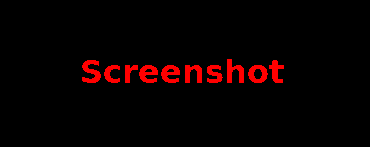
\includegraphics[width=\textwidth]{img/assignment1/screen1.png}
    \caption{Screenshot 1}\label{oswe-fig:sec2-screen1}
\end{figure}
%
%
%
\subsection{Steps Taken}\label{oswe-sec:sec2-steps}
%
...

\begin{enumerate}
    \item ...
    \item ...
    \item ...
\end{enumerate}
%
%
%
\section{Additional Information not Mentioned Above}\label{oswe-sec:last}
%
...
%
%
%
\subsection{...XYZ...}\label{oswe-sec:last-xyz}
%
... (see table \ref{oswe-tbl:last-xyz}) ...

\begin{table}[H]
    %\begin{tabularx}{\textwidth}{X|l}
    \begin{tabularx}{\textwidth}{l|l}
        \textbf{abc} & \textbf{def} \\
        \hline
        ... & ...\\
    \end{tabularx}
    \caption{XYZ\label{oswe-tbl:last-xyz}}
\end{table}
%
%
%
